\documentclass[a4paper]{report}
\usepackage{graphicx}
\usepackage{cite}
\usepackage{multirow}
\usepackage{amsmath}
\usepackage{booktabs}
\usepackage{cancel}
 \usepackage{tikz}

\def\firstcircle{(90:1.75cm) circle (2.5cm)}
\def\secondcircle{(210:1.75cm) circle (2.5cm)}
\def\thirdcircle{(330:1.75cm) circle (2.5cm)}

\usepackage{xspace}

% Add a period to the end of an abbreviation unless there's one
% already, then \xspace.
\makeatletter
\DeclareRobustCommand\onedot{\futurelet\@let@token\@onedot}
\def\@onedot{\ifx\@let@token.\else.\null\fi\xspace}

\def\eg{\emph{e.g}\onedot} \def\Eg{\emph{E.g}\onedot}
\def\ie{\emph{i.e}\onedot} \def\Ie{\emph{I.e}\onedot}
\def\cf{\emph{c.f}\onedot} \def\Cf{\emph{C.f}\onedot}
\def\etc{\emph{etc}\onedot} \def\vs{\emph{vs}\onedot}
\def\wrt{w.r.t\onedot} \def\dof{d.o.f\onedot}
\def\etal{\emph{et al}\onedot}
\makeatother

\newcommand{\ra}[1]{\renewcommand{\arraystretch}{#1}}


\bibliographystyle{apalike} 

\newcommand{\HRule}{\rule{\linewidth}{0.5mm}}

\begin{document}

\begin{titlepage}

\begin{center}

\textsc{\Large Hatch Mathematics}\\[0.5cm]

\HRule \\[0.4cm]
{\huge \bfseries Tutorial Examples}\\[0.4cm]
{\huge \bfseries Mathematics}\\[0.4cm]
\HRule \\[1.5cm]

\begin{minipage}{0.4\textwidth}
\begin{flushleft} \large
\emph{Author:}\\
Alexander \textsc{Baker}
\end{flushleft}
\end{minipage}
\begin{minipage}{0.5\textwidth}
\begin{flushright} \large
\emph{Reader:} \\
Alexander \textsc{Baker} 

\end{flushright}
\end{minipage}
\\[4cm]
\textsc{\LARGE Hatch Mathematics}\\[1.5cm]

\vfill

{\large \today}

\end{center}

\end{titlepage}

\newpage

\pagestyle{empty} %get rid of header/footer for toc page
\tableofcontents %put toc in
\cleardoublepage %start new page
\pagestyle{plain} % put headers/footers back on
\setcounter{page}{1} %reset the page counter

\newpage

\chapter{Mathematics}
\label{ch:intro}

\section{Overview}

I wanted to write some brief notes to capture the key points covered in some of our weekly tutorials. Becoming a good mathematition is possible only by applying our recently acquired mathematical knowledge. For this reason these notes include some exercises to provide the reader a chance to build some skill in applying these new mathematical facts. 

In all cases getting mathematics wrong is a part of this learning process; we expect and need to fail to efficiently learn. The only thing that separates folks whom consider themselves capable in mathematics, is the level of persistence in the presence of this inevitable and expected failure. 

We should therefore always expect to get a little bit stuck; but try, try and try again!

\section{Fractions}

The value of a fraction is unaltered if the \textit{numerator} and \textit{denominator} are multiplied or divided by the same amount. It is important that we understand the basic operations of fractions, since not only are these operations used when we are performing simplifications of numeric only examples but these also constitute the same basic operations required when tackling symbolic or algebraic manipulation.

\subsection{Addition and Subtraction}

\begin{equation}
 \frac{x}{a} + \frac{y}{b} = \frac{x \times b + y \times a}{a \times b} = \frac{xb + ya}{ab}
\end{equation}

\begin{equation}
 \frac{x}{a} - \frac{y}{b} = \frac{x \times b - y \times a}{a \times b} = \frac{xb - ya}{ab}
\end{equation}

\subsection{Multiplication and Division}

\begin{equation}
 \frac{x}{a} \times \frac{y}{b} = \frac{x \times y}{a \times b} = \frac{xy}{ab}
\end{equation}

\begin{equation}
 \frac{x}{a} \div \frac{y}{b} = \frac{x}{a} \times \frac{b}{y} = \frac{x \times b}{a \times y} = \frac{xb}{ay}
\end{equation}

\subsection{Exercise fractions}

Simplify ...

\begin{equation}
  3\frac{1}{7} + \frac{2}{3}
\end{equation}

\begin{equation}
  3\frac{1}{7} - \frac{2}{3}
\end{equation}

\begin{equation}
  \frac{3}{7} \times \frac{1}{3}
\end{equation}

\begin{equation}
  \frac{3}{7} \div \frac{7}{3}
\end{equation}

\begin{equation}
  \frac{4x}{y} \times \frac{x}{6y}
\end{equation}

\begin{equation}
  2st \times \frac{3t}{s^{2}}
\end{equation}

\begin{equation}
  \frac{4 \pi r^{2}}{3} \div 2 \pi r
\end{equation}

\begin{equation}
  \frac{4uv}{3} \div \frac{u}{2v}
\end{equation}

\begin{equation}
  \frac{\pi x^{3}}{3} \div 8 \pi x
\end{equation}

\begin{equation}
  \frac{3x^{2}}{2y} \times \frac{y}{y-2}
\end{equation}

\section{Surds and Indices}

When we express a number as the product of two equal factors, that factor is called the \textit{square root} of the number, for example $ 4 = 2 \times 2 $ thus the square root of 4 is 2. This is written as $ 2 = \sqrt{4} $. Now -2 is also a square root of 4, as $ 4 = -2 \times -2 $. We can write that $ \pm \sqrt{4} = \pm 2 $. 

\subsection{Simplifying Surds}

Consider $ \sqrt{18} $ since one of the factors of 18 is 9 and 9 has an exact square root, 

\begin{equation}
 \sqrt{18} = \sqrt{9 \times 2} = \sqrt{9} \times \sqrt{2} 
\end{equation}

However since $ \sqrt{9} = 3 $ therefore $ 3 \times \sqrt{2} $ or $ 3\sqrt{2} $. Thus $ 3\sqrt{2} $ is the simplist possible form for the surd $ \sqrt{18} $. Similarly

\begin{equation}
 \sqrt{\frac{2}{25}} = \frac{\sqrt{2}}{\sqrt{25}} = \frac{\sqrt{2}}{5} 
\end{equation}

\subsubsection{Rationalising a Surd denominator}

In the example $ \frac{2}{\sqrt{3}} $ the square root in the denominator can be removed if we multiply it by another $ \sqrt{3} $.  Thus we can apply as below:

\begin{equation}
 \frac{2}{\sqrt{3}} = \frac{2 \times \sqrt{3}}{\sqrt{3} \times \sqrt{3}} = \frac{2\sqrt{3}}{3}
\end{equation}


\subsection{Exercise surds and indices}

Simplify ...

\begin{equation}
  \frac{\sqrt{80}}{\sqrt{16}}
\end{equation}

\begin{equation}
 \left ( \frac{\sqrt{80}}{3} + \frac{1}{3} \right)
\end{equation}

\begin{equation}
 \left ( \frac{\sqrt{80}}{3} + \frac{1}{6} \right)
\end{equation}

\begin{equation}
 \left (  \frac{\sqrt{80}}{3} + 2\frac{1}{6} \right )
\end{equation}

\begin{equation}
 \left (  \frac{\sqrt{100}}{20} + \frac{1}{8} + \frac{1}{8} \right )
\end{equation}

\begin{equation}
 \left (  \frac{\sqrt{150}}{8} + 7\frac{1}{16}\right )
\end{equation}

\begin{equation}
  \frac{1}{\sqrt{7}}
\end{equation}

\begin{equation}
  \frac{2}{\sqrt{11}}
\end{equation}

\begin{equation}
  \frac{3 \sqrt{2}}{\sqrt{5}}
\end{equation}

\begin{equation}
  \frac{\sqrt{5}}{\sqrt{10}}
\end{equation}

\begin{equation}
  \frac{\sqrt{1}}{\sqrt{27}}
\end{equation}

\section{Base and Index}

In an expression such as $ 3^{4} $ the \textit{base} is 3 and the 4 is called the \textit{power} or \textit{index}, working with indices involves using some properties which apply to any base, we we express these rules in terms of a general base $a$, which stands for any number.

\subsection{Rule 1}

Because $ a^{3} $ means $ a \times a \times a $ and $ a^{2} $ means $ a \times a $ it follows that  

\begin{equation}
  a^{3} \times a^{2} = ( a \times a \times a ) \times ( a \times a ) = a^{5}
\end{equation}

More generally ...

\begin{equation}
  a^{p} \times a^{q} = a^{p + q}
\end{equation}

\subsection{Rule 2}

Dealing with division

\begin{equation}
  a^{7} \div a^{4} =\frac{\cancel{a} \times \cancel{a} \times \cancel{a}\times \cancel{a}\times a\times a\times a}{\cancel{a}\times \cancel{a}\times \cancel{a}\times \cancel{a}} = a^{3}
\end{equation}

this can be also be read as $ a^{7} \div a^{4} = a^{7-4} $ or more generally ...

\begin{equation}
  a^{p} \div a^{q} = a^{p - q}
\end{equation}

Thus from rule 2 say:

\begin{equation}
  a^{3} \div a^{5} = a^{3 - 5} = a^{-2} = \frac{1}{a^{2}}
\end{equation}

This tells us that $a^{-2}$ means $ \frac{1}{a^{2}} $ which more generally 

\begin{equation}
  a^{-p} = \frac{1}{a^{p}}
\end{equation}

This $a^{-p}$ means the reciprocal of $a^{p}$. 

Finally for rule 2 any base to the power zero is equal to 1. In fact any number at all raised to the power zero is always 1. 

\begin{equation}
  a^{0} = 1
\end{equation}

\subsection{Rule 3}

\begin{equation}
 (a^{2})^{3}  = (a \times a)^{3}
\end{equation}

\begin{equation}
(a \times a)^{3} = (a \times a) \times (a \times a) \times (a \times a)= a^{6}
\end{equation}

More generally ...

\begin{equation}
(a^{p})^{q} = a^{p \times q}
\end{equation}

Not that this is different to rule 2, since in rule 3 case we have $ (a^{p})^{q} $ where $ (a^{p})$ is raised to the power of $q$ relative to previous rule 2 case where $ a^{p} \times a^{q} $.

\subsection{Rule 4}

This rule explains the meaning of a fractional index

\begin{equation}
a^{\frac{1}{2}} \times a^{\frac{1}{2}} = a^{\frac{1}{2} + \frac{1}{2}} = a^{1} = a 
\end{equation}

Thus

\begin{equation}
a = a^{\frac{1}{2}} \times a^{\frac{1}{2}}  
\end{equation}

Therefore $a^{\frac{1}{2}}$ means $\sqrt{a} $ the positive square root of a 

\begin{equation}
a = a^{\frac{1}{2}} \times a^{\frac{1}{2}}  = \sqrt{a} \times \sqrt{a} = a^{1} = a
\end{equation}

More generally ...

\begin{equation}
a^{\frac{p}{q}} = (a^{p})^{\frac{1}{q}} 
\end{equation}

or

\begin{equation}
a^{\frac{p}{q}} = (a^{\frac{1}{q}})^{p}
\end{equation}

\subsection{Exercise base and index}

Simplify ...

\begin{equation}
  \frac{2^{3} \times 2^{7}}{4^{3}}
\end{equation}

\begin{equation}
  (x^{2})^{7} \times x^{-3}
\end{equation}


\section{Venn Diagrams and Sets}

A Venn Diagram is a pictorial representation of the relationships between sets.

$ \overline{A} \cap B$ - The intersection $\cap$ represents the overlap or overlay between two sets. It is often useful to consider these two sets separately and then try and mentally overlap these two separate diagrams. 

\subsection{$ \overline{A} \cap B$}

In the example below $ \overline{A} \cap B$ is split into two separate diagrams $ \overline{A}$ and $ B$ before we finally complete the overlap of $ \cap$ for $ \overline{A} \cap B$. Many students get confused thinking that the "overlap in the middle" represents $\cap$. This is not the case; we need to first construct both sides of the expression; in this case $ \overline{A} $ and  $B$ before we attempt to visualise where these two separate sets overlap.  As you can see from the third diagram below; this third set is more then the "bit in the middle" between the two sets.

\subsubsection{$ \overline{A}$}

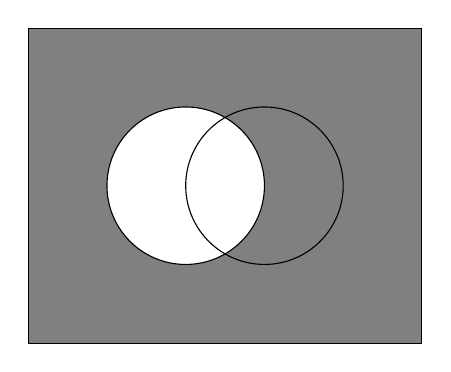
\begin{tikzpicture}
\filldraw[fill=gray] (-2,-2) rectangle (3,2);
\scope % A \cap B
\clip (0,0) circle (1);
\fill[white] (1,0) circle (2);
\endscope
% outline
\draw (0,0) circle (1)
      (1,0) circle (1);
\end{tikzpicture}

\subsubsection{$ B$}

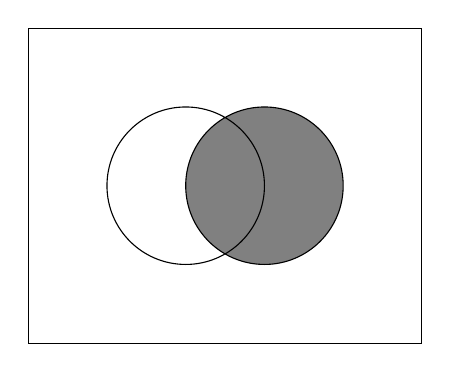
\begin{tikzpicture}
\filldraw[fill=white] (-2,-2) rectangle (3,2);
\scope % A \cap B
\clip (0,0) circle (2);
\fill[gray] (1,0) circle (1);
\endscope
% outline
\draw (0,0) circle (1)
      (1,0) circle (1);
\end{tikzpicture}

\subsubsection{$ \overline{A} \cap B$}

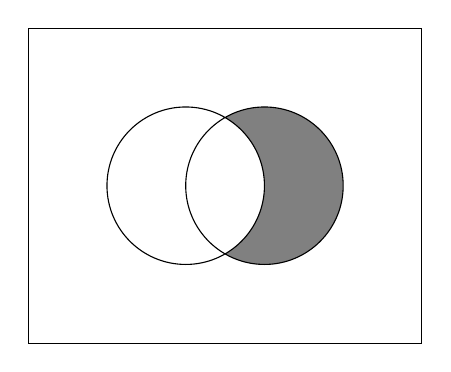
\begin{tikzpicture}
\filldraw[fill=white] (-2,-2) rectangle (3,2); 
\scope % A \cap B
\clip (0,0) circle (2);
\endscope
\scope
\clip (-1,-1) rectangle (2,1)
      (0,0) circle (1);
\fill[gray] (1,0) circle (1);
\endscope
% outline
\draw (0,0) circle (1)
      (1,0) circle (1);
\end{tikzpicture}

\subsubsection{Union $\cap$}

The union of $\cap$ between two sets is simply another way of saying that we need to add the the the two separate sets together. In the middle example shown in figure \ref{fig:example1} we can see $ a \cap B$ as everything in $A$ added or $\cap$ or Union with everything in $B$. Whilst this example is trivial; in any case where we have a $\cap$ we just need to think about shading the region from both sides of the union.

\subsubsection{Exercises}

The following figure \ref{fig:example1} show how to shade regions of Venn Diagrams for two sets:
A intersect B, A union B, A', A intersect B', A' intersect B, A union B',
A' union B, A' union B' = (A intersect B)', A' intersect B' = (A union B)'.

\begin{figure}[h]
    \centering
    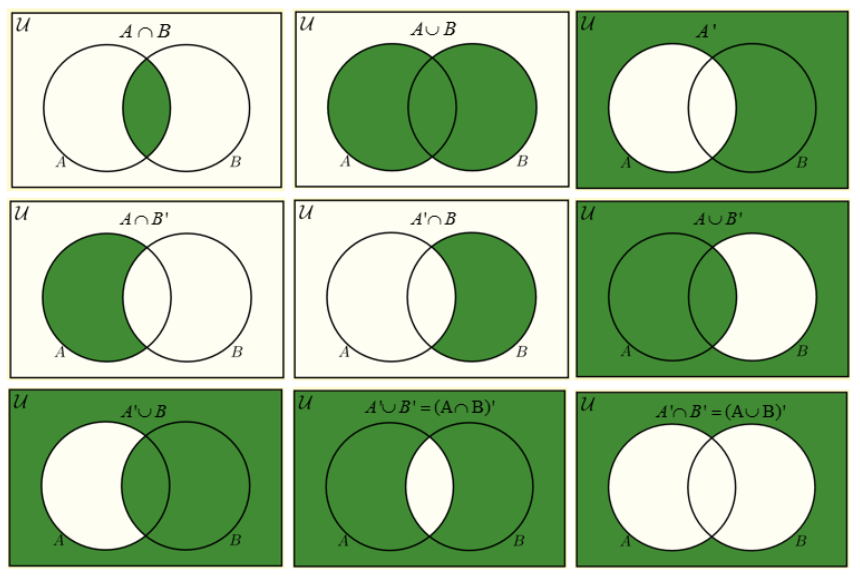
\includegraphics[width=1.25\textwidth]{set1}
    \caption{Two set examples}
    \label{fig:example1}
\end{figure}

Figure \ref{fig:example0} includes more examples of how to shade Venn Diagrams to represent the required regions of two sets and three sets where we are interested in the complement of a set.

\begin{figure}[h]
    \centering
    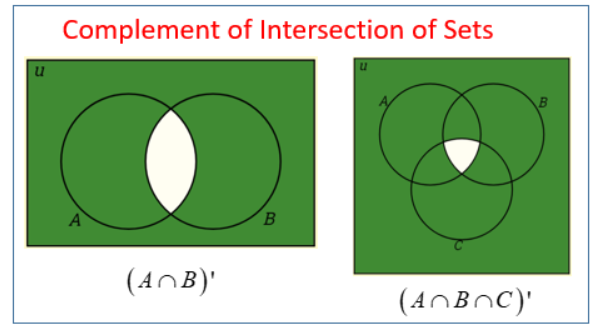
\includegraphics[width=0.95\textwidth]{set0}
    \caption{Set complement $\overline{A}$}
    \label{fig:example0}
\end{figure}

\section{Conversion of Units}

Often in examinations we are given measurements in units that are not fungible with each other. For example we want to convert $18.45 mm$ into meters or even kilometers?  We need to be able to confidently move between units of length. The notes below develop some shortcuts of heuristics based on our everyday understanding of SI units.

\subsection{Length}

We can start from the intuitive understanding from elementary maths and experience as below: 

$ 10mm \equiv 1 cm $
$ 100cm \equiv 1m $

So how does knowing these help us say convert a length of $18.45 mm$ into say meters or kilometers?  We can start by making the observation that we can manipulate any ratio in a similar way to an equation or fraction; as long as we apply the same factor to both sides of the ratio, then the same ratio remains valid. 


Using $ 10mm \equiv 1 cm $ we can safely divide both sides by 10 this giving $ \frac{10}{10}mm \equiv \frac{1}{10} cm $ which can be simplified as $ 1mm \equiv 0.1 cm $. Since we also know that $ 100cm \equiv 1m $ we can apply a similar trick as $ \frac{100}{100}cm \equiv \frac{1}{100}m $ which results in $ 1cm \equiv \frac{1}{100}m $.

Appying one final scaling to we can again $ \div 10 $ on both sides; giving us $ 0.1cm \equiv \frac{1}{1000}m $. Thus we have

$ 1mm \equiv 0.1 cm  \equiv 0.1cm \equiv \frac{1}{1000}m $. This tells us that to move from $mm$ into $m$ we just need to multiple by $\frac{1}{1000}$ or $ \times 10^{-3}$. 

Going back to the original example converting  $18.45 mm$ into meters; we just need to multiply  $18.45 \times 10^{-3} $ which gives us $0.01845 m $. We can extend this more broadly using the conversion rules shown in figure \ref{fig:convert0}.

\begin{figure}[h]
    \centering
    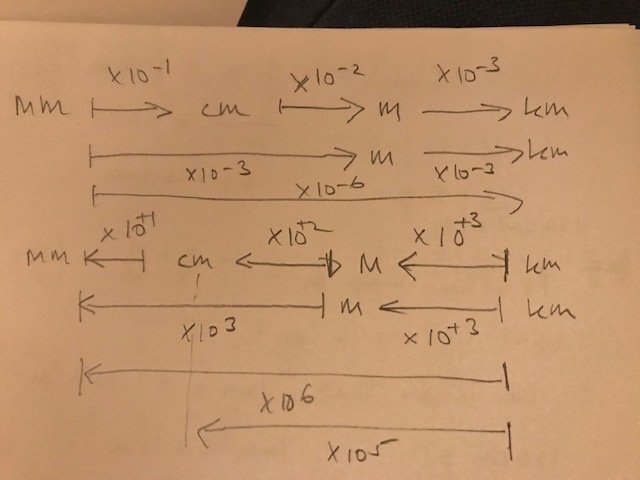
\includegraphics[width=0.75\textwidth]{IMG_2968}
    \caption{General rules to move between length units.}
    \label{fig:convert0}
\end{figure}

Figure \ref{fig:convert0} shows us the multipliers that we need to apply; for example we can use $ \times 10^{-3}$ when moving between $mm$ and $m$. However moving between $mm$ and $km$ we need $ \times 10^{-6}$. In the opposite sense if we have $km$ we can move into $m$ by $ \times 10^{+6}$. You will notice that the rules involve a simple addition of the base ten power. Moving between $mm$ to $cm$ and then $m$ and finallly $km$ involved some $ \times 10^{-6}$ separate multiplications which separately can be applied or grouped into a single $ \times 10^{-6}$ operator. 

The simplicity and beatuy of these simple unit conversions, together with the human sized $ 10mm \equiv 1 cm $ and $ 100cm \equiv 1m $ are some of the reasons why as a society we chose to make the rather painful decision to migrate to these bases.

\subsection{Conversion Examples}

One final note on unit conversion; is around the sense check that we must always apply; take the examples below, it is important for example that we analyse the sensibility of the final out come of the conversion for say  $18.45$ km to mm ; we must ask ourselves do we expect the final figure once onverted to be larger or smaller than the original. In this case clearly we have a relatively modest number of km, 18.45 in this case; of course we expect this to be a very large number of mm given the direction of conversion. Which we can gladly confirm as  $  18,450,000$ mm. However if we have made a mistake along the way; the final number might not fit with our conceptual schema and this check can operate as an important confirmation step.

\begin{itemize}
  \item \eg $18.45$ mm to meters we $(\times 10^{-3}) $ $18.45 \times 10^{-3} = 0.01845$ m
  \item \eg $18.45$ km to mm we $(\times 10^{6}) $ $18.45 \times 10^{6} = 18,450,000$ mm
  \item \eg $18.45$ m to mm we $(\times 10^{3}) $ $18.45 \times 10^{3} = 18,450 $ mm
  \item \eg $18.45$ mm to km we $(\times 10^{-6}) $ $18.45 \times 10^{-6} = 0.00001845$ km
\end{itemize}

\section{Solutions}

\subsection{Problems section 1.2.3}

\begin{equation}
  3\frac{1}{7} + \frac{2}{3} = \frac{22}{7} + \frac{2}{3} = \frac{66 + 14}{21} = \frac{80}{21}
\end{equation}

\begin{equation}
  3\frac{1}{7} - \frac{2}{3} = \frac{66 - 14}{21} = \frac{52}{21}
\end{equation}

\begin{equation}
  \frac{3}{7} \times \frac{1}{3} = \frac{3}{21} = \frac{1}{7}
\end{equation}

\begin{equation}
  \frac{3}{7} \div \frac{7}{3}  = \frac{3}{7} \times \frac{3}{7} = \frac{9}{49} = \frac{1}{9}
\end{equation}

\begin{equation}
  \frac{4x}{y} \times \frac{x}{6y} = \frac{4x{2}}{6y^{2}} = \frac{2x{2}}{3y^{2}} = \frac{2}{3} \left ( \frac{x}{y} \right )^{2}
\end{equation}

\begin{equation}
  2st \times \frac{3t}{s^{2}} = \frac{6st^{2}}{s^{2}} = \frac{6 t^{2}}{s}
\end{equation}

\begin{equation}
  \frac{4 \pi r^{2}}{3} \div 2 \pi r = \frac{4 \pi r^{2}}{3} \times \frac{1}{2 \pi r} = \frac{2r}{3}
\end{equation}

\begin{equation}
  \frac{4uv}{3} \div \frac{u}{2v} = \frac{4uv}{3} \times \frac{2v}{u} = \frac{8}{3}v^{2}
\end{equation}

\begin{equation}
  \frac{\pi x^{3}}{3} \div 8 \pi x =  \frac{\pi x^{3}}{3} \times \frac{ 1 }{8 \pi x} = \frac{x^{2}}{24}
\end{equation}

\begin{equation}
  \frac{3x^{2}}{2y} \times \frac{y}{y-2} = \frac{3}{2}  \frac{x^{2}}{ ( y-2)} 
\end{equation}

\subsection{Problems section 1.3.2}


\begin{equation}
  \frac{\sqrt{80}}{\sqrt{16}} = \frac{\sqrt{5 \times 16}}{\sqrt{16}} = 4\frac{\sqrt{5}}{4} =\sqrt{5} 
\end{equation}

\begin{equation}
 \left ( \frac{\sqrt{80}}{3} + \frac{1}{3} \right) = \left ( \frac{\sqrt{5 \times 16}}{3} + \frac{1}{3} \right) = \left ( 4\frac{\sqrt{5}}{3} + \frac{1}{3} \right) = \left ( \frac{1 + 4 \sqrt{5}}{3} \right ) = \frac{1}{3} + \frac{4 \sqrt{5}}{3} 
\end{equation}

\begin{equation}
 \left ( \frac{\sqrt{80}}{3} + \frac{1}{6} \right) =  \left ( \frac{\sqrt{5 \times 16}}{3} + \frac{1}{6} \right) = \frac{25 \sqrt{5} + 3}{18} = \frac{1}{6} + \frac{4}{3}\sqrt{5}
\end{equation}

\begin{equation}
 \left (  \frac{\sqrt{80}}{3} + 2\frac{1}{6} \right ) =  \left (  \frac{\sqrt{5 \times 16}}{3} + \frac{13}{6} \right ) = \frac{24 \sqrt{5} + 39}{18} = \frac{39}{18} + \frac{4}{3} \sqrt{5}
\end{equation}

\begin{equation}
 \left (  \frac{\sqrt{100}}{20} + \frac{1}{8} + \frac{1}{8} \right )
\end{equation}

\begin{equation}
 \left (  \frac{\sqrt{150}}{8} + 7\frac{1}{16}\right ) = \frac{10}{20} + \frac{2}{8} = \frac{1}{2} + \frac{1}{4} = \frac{3}{4}
\end{equation}

\begin{equation}
  \frac{1}{\sqrt{7}} =  \frac{\sqrt{7}}{\sqrt{7} \times \sqrt{7}} = \frac{\sqrt{7}}{7}
\end{equation}

\begin{equation}
  \frac{2}{\sqrt{11}} = \frac{2 \sqrt{11}}{11}
\end{equation}

\begin{equation}
  \frac{3 \sqrt{2}}{\sqrt{5}} = \frac{3 \sqrt{2} \times \sqrt{5}}{\sqrt{5} \times \sqrt{5}} = \frac{3 \sqrt{2} \times \sqrt{5}}{5} = \frac{3 \sqrt{10}}{5} = \frac{3}{5}\sqrt{10}
\end{equation}

\begin{equation}
  \frac{\sqrt{5}}{\sqrt{10}} = \frac{\sqrt{5} \sqrt{10}}{\sqrt{10}\sqrt{10}} = \frac{\sqrt{50}}{10} = \frac{1}{10} \sqrt{2 \times 25} = \frac{\sqrt{2}}{2}
\end{equation}

\begin{equation}
  \frac{\sqrt{1}}{\sqrt{27}} = \frac{\sqrt{\sqrt{27}}}{27}
\end{equation}

\subsection{Problems section 1.4.5}

\begin{equation}
  \frac{2^{3} \times 2^{7}}{4^{3}} = \frac{2^{10}}{4^{3}} = \frac{2^{10}}{2^{6}} = 2^{10} \times 2^{-6} = 2^{4}
\end{equation}

\begin{equation}
  (x^{2})^{7} \times x^{-3} = \frac{x^{14}}{x^{3}} = x^{14-3} = x^{11}
\end{equation}



\section{Quadratic Equations}

A number of separate techniques exist for solving equations that are of the form $ ax^{2} +bx + c = 0 $ some methods are quite simple and others whilst less simple are more beautiful. None less beautiful than completing the square coupled with a geometic explanation as shown in the next section.

\subsection{Completing the Square}


\begin{figure}[h]
    \centering
    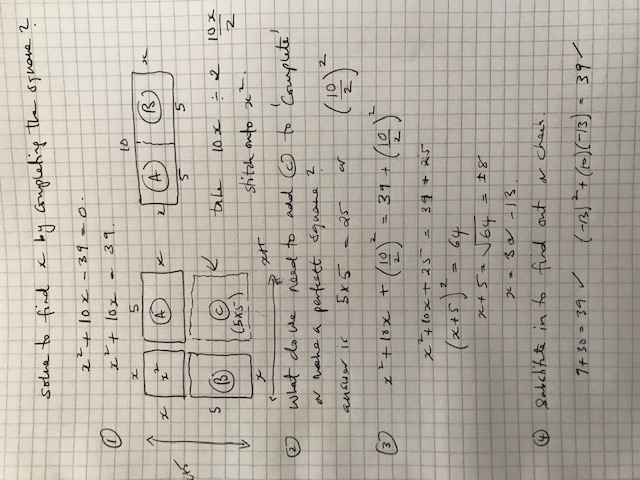
\includegraphics[width=1.25\textwidth]{IMG_3049}
    \caption{Complete Example - Completing the Square}
    \label{fig:example1}
\end{figure}

\begin{figure}[h]
    \centering
    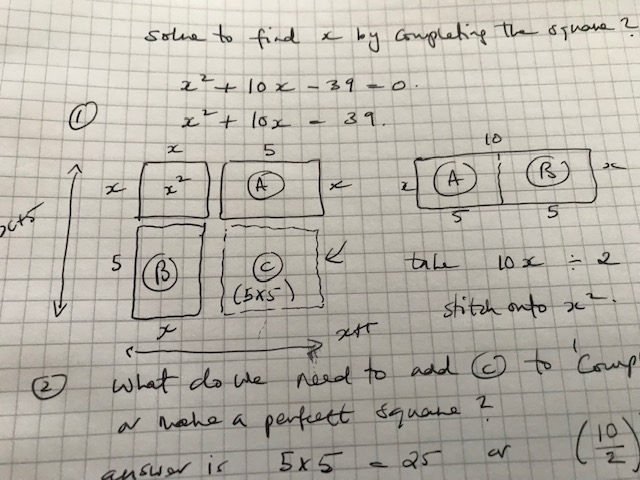
\includegraphics[width=1.25\textwidth]{IMG_3050}
    \caption{Two set examples}
    \label{fig:example1}
\end{figure}


\end{document}
